\documentclass{article}\usepackage[]{graphicx}\usepackage[]{color}
%% maxwidth is the original width if it is less than linewidth
%% otherwise use linewidth (to make sure the graphics do not exceed the margin)
\makeatletter
\def\maxwidth{ %
  \ifdim\Gin@nat@width>\linewidth
    \linewidth
  \else
    \Gin@nat@width
  \fi
}
\makeatother

\definecolor{fgcolor}{rgb}{0.345, 0.345, 0.345}
\newcommand{\hlnum}[1]{\textcolor[rgb]{0.686,0.059,0.569}{#1}}%
\newcommand{\hlstr}[1]{\textcolor[rgb]{0.192,0.494,0.8}{#1}}%
\newcommand{\hlcom}[1]{\textcolor[rgb]{0.678,0.584,0.686}{\textit{#1}}}%
\newcommand{\hlopt}[1]{\textcolor[rgb]{0,0,0}{#1}}%
\newcommand{\hlstd}[1]{\textcolor[rgb]{0.345,0.345,0.345}{#1}}%
\newcommand{\hlkwa}[1]{\textcolor[rgb]{0.161,0.373,0.58}{\textbf{#1}}}%
\newcommand{\hlkwb}[1]{\textcolor[rgb]{0.69,0.353,0.396}{#1}}%
\newcommand{\hlkwc}[1]{\textcolor[rgb]{0.333,0.667,0.333}{#1}}%
\newcommand{\hlkwd}[1]{\textcolor[rgb]{0.737,0.353,0.396}{\textbf{#1}}}%

\usepackage{framed}
\makeatletter
\newenvironment{kframe}{%
 \def\at@end@of@kframe{}%
 \ifinner\ifhmode%
  \def\at@end@of@kframe{\end{minipage}}%
  \begin{minipage}{\columnwidth}%
 \fi\fi%
 \def\FrameCommand##1{\hskip\@totalleftmargin \hskip-\fboxsep
 \colorbox{shadecolor}{##1}\hskip-\fboxsep
     % There is no \\@totalrightmargin, so:
     \hskip-\linewidth \hskip-\@totalleftmargin \hskip\columnwidth}%
 \MakeFramed {\advance\hsize-\width
   \@totalleftmargin\z@ \linewidth\hsize
   \@setminipage}}%
 {\par\unskip\endMakeFramed%
 \at@end@of@kframe}
\makeatother

\definecolor{shadecolor}{rgb}{.97, .97, .97}
\definecolor{messagecolor}{rgb}{0, 0, 0}
\definecolor{warningcolor}{rgb}{1, 0, 1}
\definecolor{errorcolor}{rgb}{1, 0, 0}
\newenvironment{knitrout}{}{} % an empty environment to be redefined in TeX

\usepackage{alltt}
\usepackage[margin=0.75in]{geometry}
\usepackage{amsmath,amssymb}
\usepackage{graphicx,float}
\usepackage{multirow,setspace}
\usepackage{enumerate}
\usepackage{booktabs}
\usepackage{placeins}
\usepackage{cite}
\usepackage{caption}
\usepackage{subcaption}
\usepackage{wrapfig}
\usepackage{hyperref}
\usepackage{listings}

\newcommand{\HRule}{\rule{\linewidth}{0.5mm}}
\newcommand{\tab}{\hspace{0.5cm}}
\newcommand{\modref}[1]{(\ref{#1})}
\mathchardef\mhyphen="2D




\newcounter{DefnCounter}
\setcounter{DefnCounter}{1}

\newcounter{ThmCounter}
\setcounter{ThmCounter}{1}

\newcounter{ExampleCounter}
\setcounter{ExampleCounter}{1}

\newcommand{\defn}[1]{\textsc{Definition 1.\arabic{DefnCounter}\stepcounter{DefnCounter}: #1\\} }
\newcommand{\thm}{\textsc{Theorem 1.\arabic{ThmCounter}\stepcounter{ThmCounter}\\} }
\newcommand{\ex}{\textsc{Example 1.\arabic{ExampleCounter}\stepcounter{ExampleCounter}\\} }

\newcommand{\Defn}{\underline{Definition}}
\newcommand{\Q}{\underline{Question}}
\newcommand{\Qs}{\underline{Questions}}
\newcommand{\bbeta}{{\mbox{\boldmath$\beta$}}}
\newcommand{\bmu}{{\mbox{\boldmath$\mu$}}}
\newcommand{\balpha}{{\mbox{\boldmath$\alpha$}}}
\newcommand{\btheta}{{\mbox{\boldmath$\theta$}}}
\newcommand{\bphi}{{\mbox{\boldmath$\phi$}}}
\newcommand{\bSigma}{{\mbox{\boldmath$\Sigma$}}}
\newcommand{\bLambda}{{\mbox{\boldmath$\Lambda$}}}
\newcommand{\bpi}{{\mbox{\boldmath$\pi$}}}
\newcommand{\R}{\texttt{R}}
\newcommand{\Lik}{\mathcal{L}}
\newcommand{\bx}{\textbf{x}}
\newcommand{\by}{\textbf{y}}
\newcommand{\bX}{\textbf{X}}
\newcommand{\sic}{\text{Inv-}\chi^2}


\newcommand{\sao}{SaO$_2$}

\setlength{\marginparwidth}{2cm}
\IfFileExists{upquote.sty}{\usepackage{upquote}}{}
\begin{document}


\begin{center}
	\vspace{0.1cm}
	\textsc{\LARGE MATH 640 Final Project} \\[0.1cm]
	Jason Michaels (jam521), Niko Paulson (ndp32), Miranda Seitz-McLeese (mgs85) 
\end{center}
\section{Introduction}
\label{s:intro}
This analysis will be done on a data set of a variety of measurements about severe weather in the United States. 
We chose to use a subset of that data covering the years 1996 through 2016. The data coms from the NOAA website \cite{dataset}. For this project we focused on the deaths directly attributable to a type of weather event. In the interest of time, we limited our models to two types of severe weather, Tornados and Flash Floods, reponsible for the second and third most direct deaths among weather types. Understanding how and at what rate severe weather events become lethal in the United States has tremendous public health impacts. In this paper we compare four possible models for the deaths: The traditional Poisson and negative binomial distributions, as well as the zero inflated variant of each. 

The remainder of this analysis is organized as follows: Section~\ref{s:methods} discusses and derives the models. Section~\ref{s:results} describes the results of the analysis. And Section~\ref{s:discussion} contains the conclusions.

\section{Methods}
\label{s:methods}
The deaths attributed to a severe weather event is `count' data. 
The most common model used for count data is the Poisson distribution. 
However for some weather events, the negative binomial model is a better fit, because the Poisson distribution assumes that the events being counted occur independently.

Fortunately, the vast majority of severe weather events in the United States involve no deaths, therefore we wanted to also account for the possibility of structural zeros, therefore we also considered zero inflated variants. 
These distributions are created by returning $0$ with probability $\sigma$ and sampling from the original distribution with probability $(1-\sigma)$. We will derive and fit a model for each of the four distributions and see if there is a difference in our results and evaluate to determine which model best fits the data.

\subsection{Poisson}
\label{ss:mPoisson}
The Poisson model has one parameter, $\lambda$ represents the expected number of occurances of the event of interest. For a single random variable $x$, the probability density is:
$$p(x|\lambda)=\frac{\lambda^xe^{-\lambda}}{x!}.$$
Thus the likelihood for a sum of Poisson random variables can be written as follows:
$$\mathcal{L}(X|\lambda)\propto\lambda^{n\bar{X}}e^{-n\lambda}.$$ 
Since we want the data to speak for itself, we will use a non-informative random variable, namely, Jeffreys' prior. For the Poisson distribtion this is given as follows:
$$\pi(\lambda)\propto\lambda^{1/2-1}e^{-0\cdot\lambda}.$$
We recognize this as the kernel of an improper gamma distribution. Combining the likelihood and the prior distribtion yields the following posterior distribution:
$$p(\lambda|X)=\lambda^{n\bar{X}+1/2-1}e^{-n\lambda}.$$
We recognize this as the kernel of a gamma distribution, namely
$$\lambda|X\sim\mathcal{G}amma(n\bar{X}+1/2,n).$$

\subsection{Negative Binomial}
\label{ss:mNBinom}
The Negative Binomial model has two parameters, $r,p$ represents the expected number of occurances of the event of interest. For a single random variable $x$, the probability density is:
$$p(X|r,p)=\frac{\Gamma(r+x)}{\Gamma(r)x!}p^{x}(1-p)^{r}.$$

Thus the likelihood for a sum of Negative Binomial random variables can be written as follows:
$$\mathcal{L}(X|r,p)=\Bigg[\prod_{i=1}^n\frac{\Gamma(r+x_i)}{\Gamma(r)x_i!}\Bigg]p^{n\bar{X}}(1-p)^{nr}.$$
Since we want the data to speak for itself, we will use a non-informative random variable, namely, Jeffreys' prior. For the Poisson distribtion this is given as follows:
$$\pi(r,p)=r^{1/2}p^{-1}(1-2)^{-1/2}.$$
Combining the likelihood and the prior distribtion yields the following posterior distribution:
$$p(r,p|X)=\Bigg\{\Bigg[\prod_{i=1}^n\frac{\Gamma(r+x_i)}{\Gamma(r)x_i!}\Bigg]p^{n\bar{X}}(1-p)^{nr}\Bigg\}\Bigg\{r^{1/2}p^{-1}(1-2)^{-1/2}\Bigg\}$$
From this posterior we obtain the full conditionals. First consider $p|r,X$:
$$p(p|r,X)\propto p^{n\bar{x}-1}(1-p)^{nr+1/2-1}$$
We recognize this as the kernel of a beta distribution, namely

$$p|r,X\sim\mathcal{B}eta(n\bar{X},nr+1/2).$$
Next consider $r|p,X$:
$$p(r|p,X)\propto\bigg[\prod_{i=1}^n\Gamma(r+x_i)\bigg]\Gamma(r)^{-n}(1-p)^{nr}r^{1/2}$$
This is not a recognized distribtion. So if we wish to make inferences on $r$ we must use a Metropolis algorithm to sample from it.

\subsection{Zero Inflated Poisson}
\label{ss:mZiPoisson}
The Zero Inflated Poisson (ZIP) model has two parameters. The parameter p is the probability of a structural zero, and $\lambda$ corresponds to the parameter in a typical Poisson model. For a single observation x, the probability density is:

\[
p(x|p, \lambda) = pI_{x=0}(x) + (1-p)\frac{e^{-\lambda}\lambda^x}{x!}
\]
 
 
\noindent We can write the likelihood as follows:
$$
L(p, \lambda|X) = \prod_{x_i=0}\bigg[p+(1-p)\frac{e^{-\lambda}\lambda^{x_i}}{x_i!}\bigg]\prod_{x_i \ne 0}\bigg[(1-p)\frac{e^{-\lambda}\lambda^{x_i}}{x_i!}\bigg]
$$

\noindent Bayarri, Berger, and Datta (2008) suggest using the prior distribution $\pi(\lambda, p) \propto \frac{1}{\sqrt{\lambda}}I(0<p<1)$. This gives us the following posterior 

\[
\prod_{x_i=0}\bigg[p+(1-p)\frac{e^{-\lambda}\lambda^{x_i}}{x_i!}\bigg]\prod_{x_i \ne 0}\bigg[(1-p)\frac{e^{-\lambda}\lambda^{x_i - 1/2}}{x_i!}\bigg]
\]

\noindent Neither of the full conditional distributions is recognizable (see \ref{a:dZIP}). We can use a Metropolis-Hastings algorithm to sample from both of them. We will use a beta distribution as a proposal for p, and a gamma for $\lambda$. We will tune them to obtain a better acceptance rate. 


\subsection{Zero Inflated Negative Binomial}
\label{ss:mZiNBinom}
The Zero Inflated Negative Binomial (ZINB) model has three parameters $\sigma,$ the probability of a structural zero, and $p,r$ the usual negative binomial parameters. 
For a single $X$ the probability density is: 
$$p(X|\sigma, p, r) = \sigma I_{X=0}(X) + (1-\sigma)\frac{\Gamma(r+X)}{\Gamma(r)X!}p^X(1-p)^r.$$
We take the uniform priors for $\sigma$ and $p$ as well as the non-informative gamma for $r$ which is $r^{-1/2}$. For a full derivation, see \ref{a:dZINB}. My posterior is:
$$p(r,\sigma, p|X)\propto\left(\sigma + (1-\sigma)(1-p)^r\right)^Z(1-\sigma)^{N-Z}(1-p)^{(N-Z)r}p^{\sum_{i=1}^NX_i}r^{-1/2}\prod_{i=1}^N\left(\frac{\Gamma(r+X_i)}{\Gamma(r)}\right)$$
This distribution does not factor nicely, so I will use the Metropolis algorithm to sample from it. Because this posterior does not suggest any obvious proposal distributions I will sample each independently from a normal distribution centered at $\theta^*$, and with a variance that is tuned to yield an appropriate acceptance rate.

\section{Results}
\label{s:results}
\subsection{Poisson}
\label{ss:rPoisson}

Because the posterior from our Poisson likelihood and noninformative prior had a recognizable kernel, namely $\mathcal{G}amma(n\bar{X}+1/2,n)$, we were able to sample from this distribution directly. For both Tornados, and Flash Floods, 10,000 samples were taken, to simulate the variable of interest, $\lambda$. The results are summarized in Table~\ref{t:rPOIS}, while density plots can be found in Figure~\ref{f:poisdensity}.

\begin{table}
    \centering
    \caption{Posterior distributions of $\lambda$, for both event types. The second column relays the median of the sample for $\lambda$, with the 95 percent credible interval in parentheses.}
    \label{t:rPOIS}
    \begin{tabular}{| l | l | l |}
    \hline
    Event Type & $\lambda$  \\ \hline
    Tornado & 0.0592 (0.0564, 0.0620) \\ \hline
    Flash Flood & 0.0179 (0.0170, 0.0189) \\ \hline
    \end{tabular}
\end{table}

\begin{figure}[p]
\centering
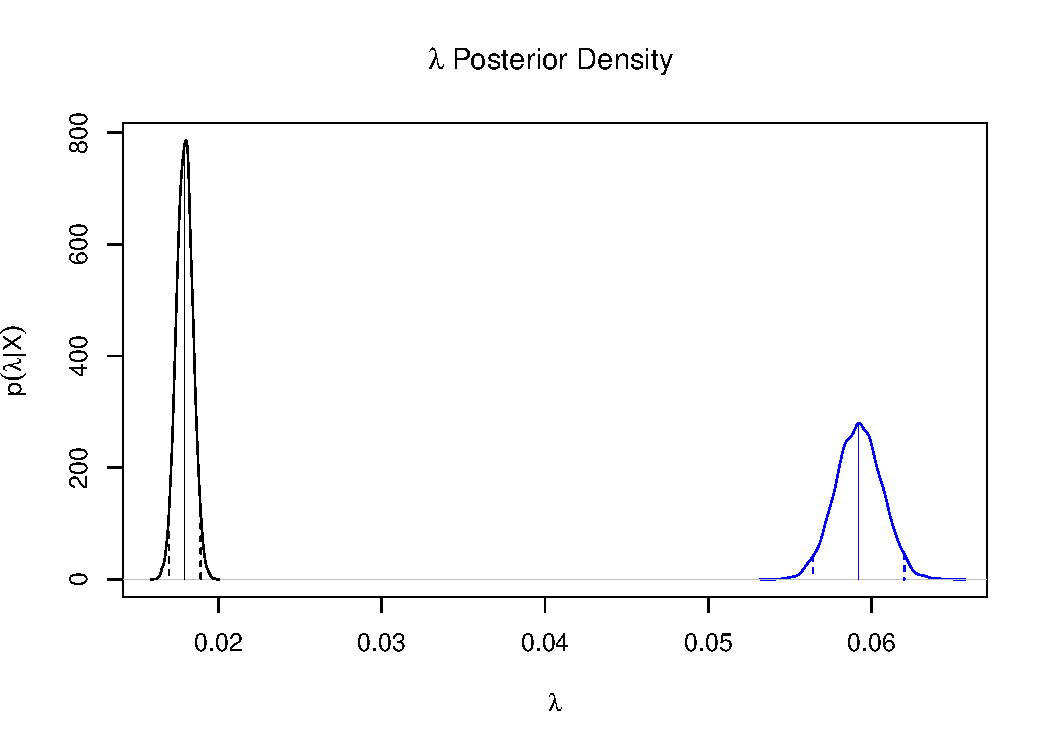
\includegraphics[width=.65\textwidth]{figure/POIS_Density.pdf}
\caption{Posterior density plots (Poisson model) for flood parameters (in blue), and tornado parameters (black). The solid line represents the median and the dashed lines indicate the 95\% confidence interval.}
\label{f:poisdensity}
\end{figure}

\subsection{Negative Binomial}
\label{ss:rNBinom}

As in the case of the Poisson distribution, the conditional posterior from our Negative Binomial likelihood and noninformative prior had a recognizable kernel for $p$, namely $\mathcal{B}eta(n\bar{X},nr+1/2)$, thus we were able to sample from this distribution directly. Meanwhile we took $r$ as known. For both Tornados, and Flash Floods, 10,000 samples were taken, to simulate the variable of interest, $p$. The results are summarized in Table~\ref{t:rNB}, while density plots can be found in Figure~\ref{f:nbdensity}.

\begin{table}
    \centering
    \caption{Posterior distributions of $p$, for both event types. The second column relays the median of the sample for $p$, with the 95 percent credible interval in parentheses.}
    \label{t:rNB}
    \begin{tabular}{| l | l | l |}
    \hline
    Event Type & $p$  \\ \hline
    Tornado & 0.0559 (0.0534, 0.0585) \\ \hline
    Flash Flood & 0.0176 (0.0167, 0.0186) \\ \hline
    \end{tabular}
\end{table}

\begin{figure}[p]
\centering
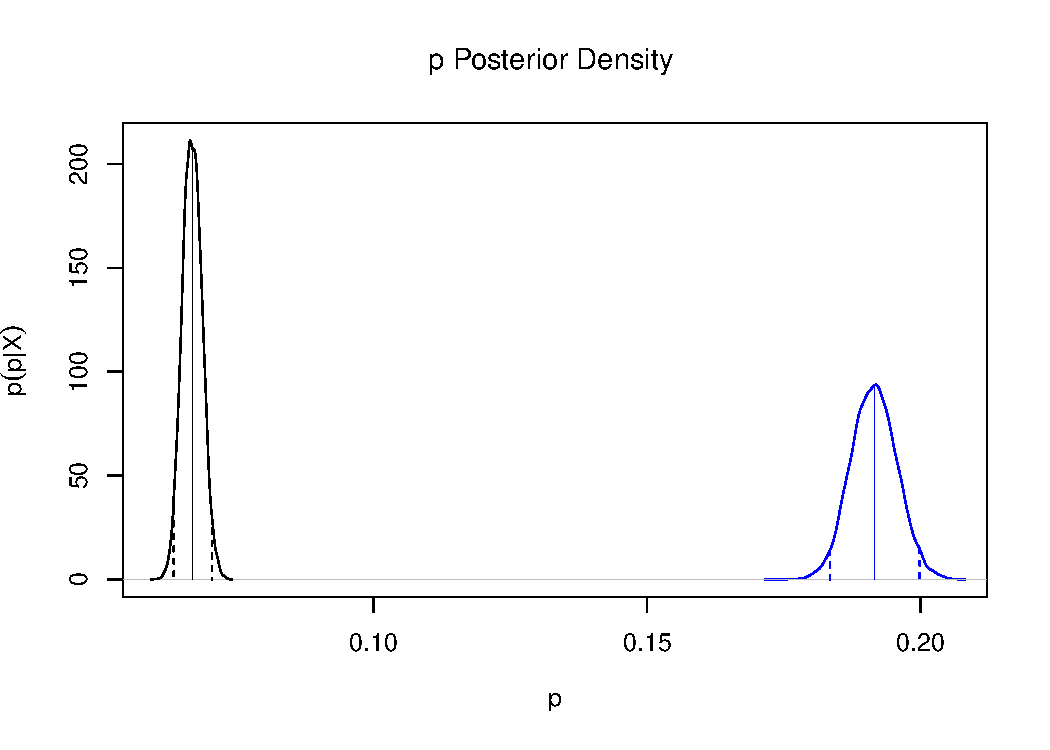
\includegraphics[width=.65\textwidth]{figure/NB_Density.pdf}
\caption{Posterior density plots (Negative Binomial model) for flood parameters (in blue), and tornado parameters (black). The solid line represents the median and the dashed lines indicate the 95\% confidence interval.}
\label{f:nbdensity}
\end{figure}

\subsection{Zero Inflated Poisson}
\label{ss:rZiPoisson}

In tuning the parameters of the two models, slightly different values were chosen for the two different event types. The proposal distribution selected for $\lambda$ was a gamma(2, 2) for tornados, and a gamma(1, 2) for flash floods. The proposal for p within the tornado model was a beta(1940, 60), whereas it was a beta(2945, 55) in the flash flood model. 

For each variable of interest, 20,000 samples were taken. As convergence was not immediately achieved, the first 10,000 samples were discarded as a burn-in. The results are summarized in Table~\ref{t:rZIP}. Convergance plots can be found in Figure~\ref{f:zipconv}, and density plots can be found in Figure~\ref{f:zipdensity}.

\begin{table}
    \centering
    \caption{The posterior distributions of $\lambda$ and p, for both event types. The second column relays the mean of the sample for $\lambda$, with the 95 percent credible interval in parentheses. The third does the same for p.}
    \label{t:rZIP}
    \begin{tabular}{| l | l | l |}
    \hline
    Event Type & $\lambda$ & p  \\ \hline
    Tornado & 1.872 (1.030, 3.710) & 0.971 (0.968, 0.973) \\ \hline
    Flash Flood & 0.562 (0.293, 0.972) & 0.982 (0.981, 0.983) \\ \hline
    \end{tabular}
\end{table}

\begin{figure}[p]
\centering
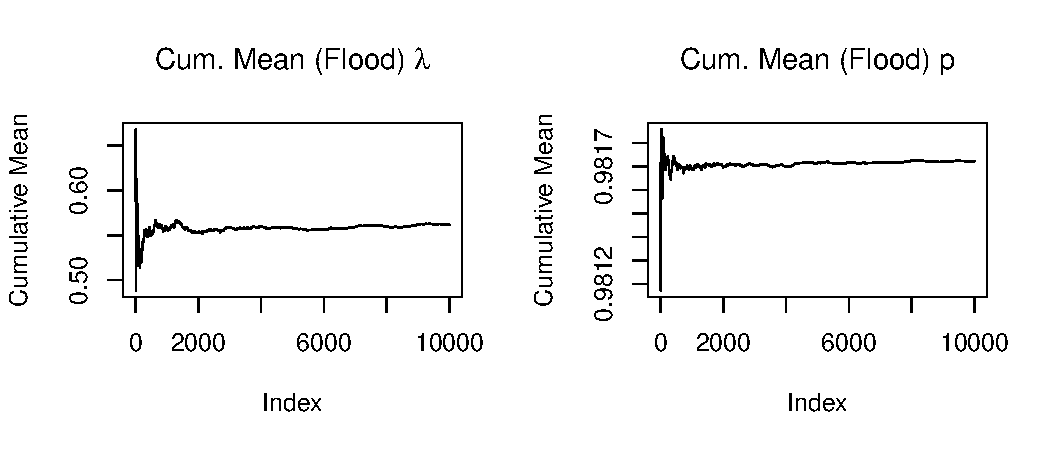
\includegraphics[width=.65\textwidth]{figure/ZIP_Flood_Conv.pdf}
\caption{Cumulative mean plots for the posterior samples (ZIP model) of the two parameters from the flood data. Plots for the tornado data are not pictured, but behave similarly.}
\label{f:zipconv}
\end{figure}

\begin{figure}[p]
\centering
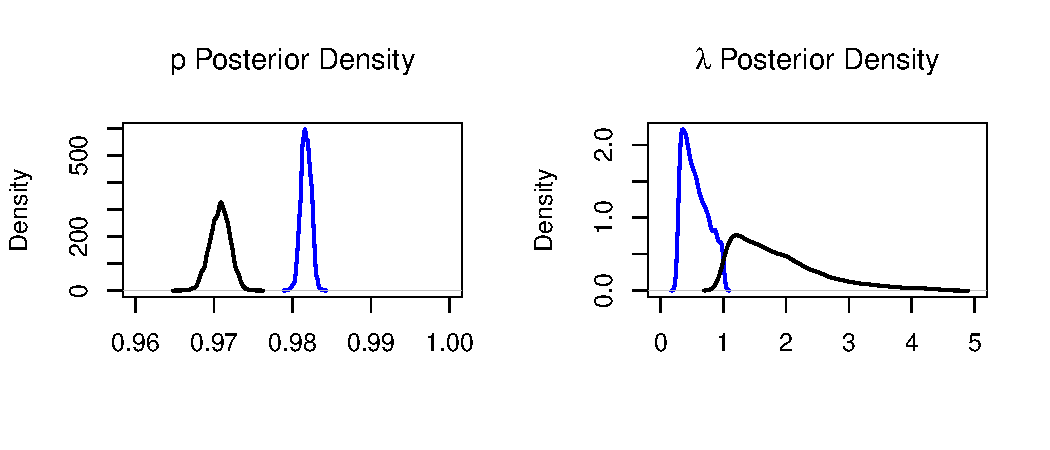
\includegraphics[width=.65\textwidth]{figure/ZIP_Density.pdf}
\caption{Posterior density plots (ZIP model) for flood parameters (in blue), and tornado parameters (black). The solid line represents the mean and the dashed lines indicate the 95\% confidence interval.}
\label{f:zipdensity}
\end{figure}

\subsection{Zero Inflated Negative Binomial}
\label{ss:rZiNBinom}



The ZINB model was fit using the Metropolis-Hastings algorithm with a multivariate truncated normal distribution used as the proposal distribution. For the source code of the sampler, please see \ref{a:cZINB}.

This model suffered severely from the curse of dimensionality. It was very slow to converge, and the very small variance needed for a reasonable acceptance led to high autocorrelation, meaning agressive thinning was necessary. Running mean plots the Flash Flood models can be found in Figure~\ref{f:zinbconvergence}. 


In the end $1030000$ samples were drawn for each model, with a burn in of $30000$ and one of every $100$ samples was retained, resulting in a final sample size of $10000$. The flood model had an acceptance rate of $0.195$ and the tornado model had an acceptance rate of $0.195$. The resulting densities are pictured in Figure~\ref{f:zinbdensity}, and Table~\ref{t:ZINBparams}, though due to questions of convergence the results should viewed with caution.



The DIC for floods and tornadoes respectively were $10804$ and $7166$.
\begin{table}
\centering
\caption{The following table shows the results of the flash flood ZINB model and the tornado ZINB model. It shows the mean and the median for each parameter as well as the 95\% credible interval.}
\label{t:ZINBparams}
\begin{tabular}{lcccccc}
\toprule
&\multicolumn{3}{c}{Flash Flood}&\multicolumn{3}{c}{Tornado}\\
\cmidrule(r){2-4}\cmidrule(l){5-7}
Parameter & Mean Value &Median Value & (95\% CI)& Mean Value &Median Value & (95\% CI)\\
\midrule
$\sigma$ & 0.307 &
  0.282&
  (0.013, 
    0.716)&
  0.299 &
  0.276&
  (0.012, 
    0.702)\\
$p$ &  0.554 &
  0.555&
  (0.518, 
    0.589)&
  0.862 &
  0.863&
  (0.841, 
    0.882)\\
$r$ &  0.024 &
  0.02&
  (0.014, 
    0.052)&
  0.015 &
  0.013&
  (0.009, 
    0.033)\\
\bottomrule
\end{tabular}
\end{table}
\begin{figure}[p]
	\centering
\begin{knitrout}
\definecolor{shadecolor}{rgb}{0.969, 0.969, 0.969}\color{fgcolor}
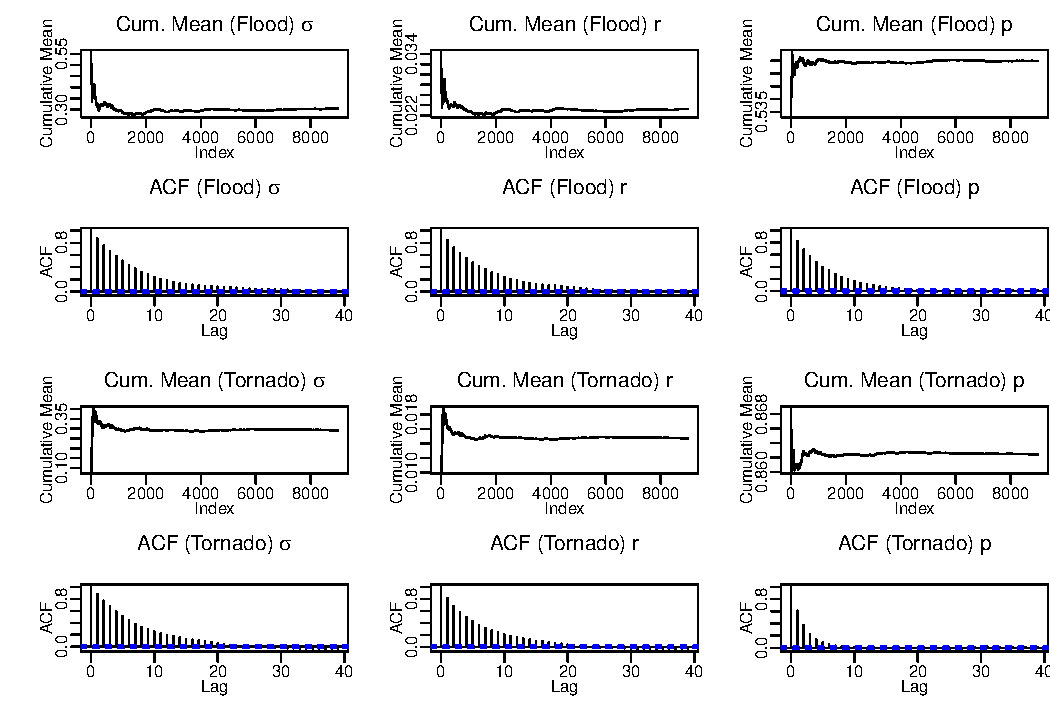
\includegraphics[width=\maxwidth]{figure/floodconvergence-1} 

\end{knitrout}
	\caption{Cumulative mean plots for each of the three parameters in the ZINB model fit on flash flood data. The tornado plots are not pictured, but are similar in character.}
	\label{f:zinbconvergence}
\end{figure} 

\begin{figure}[p]
	\centering
\begin{knitrout}
\definecolor{shadecolor}{rgb}{0.969, 0.969, 0.969}\color{fgcolor}
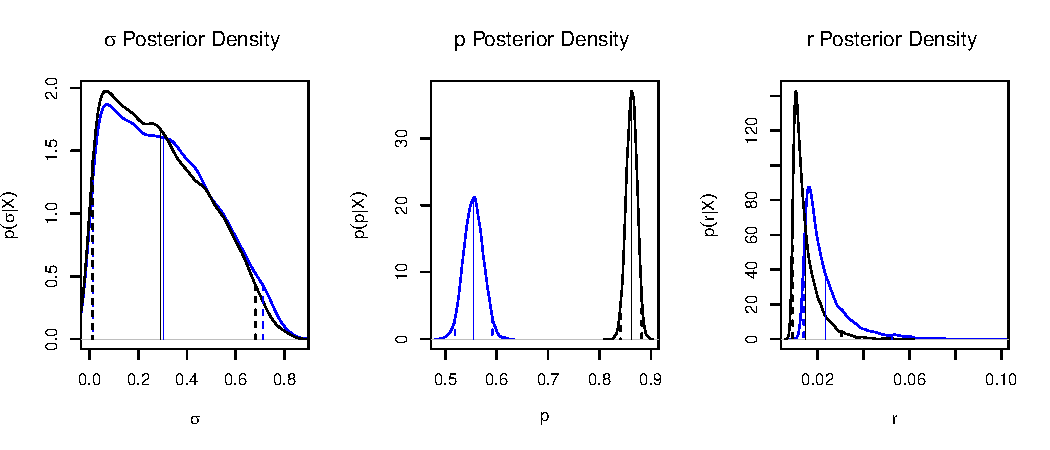
\includegraphics[width=\maxwidth]{figure/zinbdensity-1} 

\end{knitrout}
	\caption{Posterior density curves for each of the three variables. The flood posterior is shown in blue and the tornado posterior is shown in black.}
	\label{f:zinbdensity}
\end{figure} 
\section{Discussion}
\label{s:discussion}
The goal of this analysis was to determine which of the four models was the best fit for the data. In order to make this determination the DIC was calculated for each model on both tornados and flash floods. The results are summarized in Table~\ref{t:evalresults}.

\begin{table}
\centering
\caption{The following table shows the resulting DIC for each of the four models on both the tornado data and the flash flood data.}
\label{t:evalresults}
\begin{tabular}{lcc}
\toprule
Model & DIC Flash Flood & DIC Tornado\\
\midrule
Poisson & 14237 & 17606\\
Negative Binomial & 101548 & 26372\\
ZIP & 10454 & 8727 \\
ZINB & 10804.104&7166.309\\
\bottomrule
\end{tabular}
\end{table}

In general, models with smaller DIC are preferred to models with larger DIC. From the table we can see that the Zero Inflated Poisson model has the lowest DIC, both for Flash Floods and Tornados. Thus for estimating the rate of leathality of Flash Floods, Tornados, and possibly other severe weather, we should use a Zero Inflated Poisson model to fit the data. 

\clearpage
\begin{thebibliography}{2}
  \bibitem{dataset} NOAA's Severe Weather Data Inventory, 
    \url{https://www1.ncdc.noaa.gov/pub/data/swdi/stormevents/csvfiles/}. 
    Accessed April 2017.
  \bibitem{ZIP} Bayarri, M., Berger, J., Datta, G. (2008). Objective testing of Poisson versus inflated Poisson models. IMS 	Collections, 3, 105-121. 
\end{thebibliography}

\appendix
\section{Code}
\label{a:code}
This appendix includes the code used to implement the models.
\subsection{Zero Inflated Negative Binomial code}
\label{a:cZINB}
\begin{knitrout}
\definecolor{shadecolor}{rgb}{0.969, 0.969, 0.969}\color{fgcolor}\begin{kframe}
\begin{alltt}
\hlstd{logpost} \hlkwb{<-} \hlkwa{function}\hlstd{(}\hlkwc{sigma}\hlstd{,} \hlkwc{p}\hlstd{,} \hlkwc{r}\hlstd{,} \hlkwc{Z}\hlstd{,} \hlkwc{N}\hlstd{,} \hlkwc{S}\hlstd{,} \hlkwc{nonzero}\hlstd{)\{}
  \hlstd{lp} \hlkwb{<-} \hlstd{Z}\hlopt{*}\hlkwd{log}\hlstd{(}\hlnum{1} \hlopt{+} \hlstd{(}\hlnum{1}\hlopt{/}\hlstd{sigma}\hlopt{-}\hlnum{1}\hlstd{)}\hlopt{*}\hlstd{(}\hlnum{1}\hlopt{-}\hlstd{p)}\hlopt{^}\hlstd{r)}
  \hlstd{lp} \hlkwb{<-} \hlstd{lp} \hlopt{+} \hlstd{Z}\hlopt{*}\hlkwd{log}\hlstd{(sigma)}
  \hlstd{lp} \hlkwb{<-} \hlstd{lp} \hlopt{+} \hlstd{(N}\hlopt{-}\hlstd{Z)}\hlopt{*}\hlkwd{log}\hlstd{(}\hlnum{1}\hlopt{-}\hlstd{sigma)}
  \hlstd{lp} \hlkwb{<-} \hlstd{lp} \hlopt{+} \hlstd{(N}\hlopt{-}\hlstd{Z)}\hlopt{*}\hlstd{r}\hlopt{*}\hlkwd{log}\hlstd{(}\hlnum{1}\hlopt{-}\hlstd{p)}
  \hlstd{lp} \hlkwb{<-} \hlstd{lp} \hlopt{+} \hlstd{S}\hlopt{*}\hlkwd{log}\hlstd{(p)}
  \hlstd{lp} \hlkwb{<-} \hlstd{lp} \hlopt{-} \hlkwd{log}\hlstd{(r)}\hlopt{/}\hlnum{2}
  \hlstd{lp} \hlkwb{<-} \hlstd{lp} \hlopt{-} \hlstd{(N}\hlopt{-}\hlstd{Z)}\hlopt{*}\hlkwd{lgamma}\hlstd{(r)}
  \hlstd{lp} \hlkwb{<-} \hlstd{lp} \hlopt{+} \hlkwd{sum}\hlstd{(}\hlkwd{lgamma}\hlstd{(r}\hlopt{+}\hlstd{nonzero))}
  \hlkwd{return}\hlstd{(lp)}
\hlstd{\}}

\hlstd{loglik} \hlkwb{<-} \hlkwa{function}\hlstd{(}\hlkwc{sigma}\hlstd{,} \hlkwc{p}\hlstd{,} \hlkwc{r}\hlstd{,} \hlkwc{Z}\hlstd{,} \hlkwc{N}\hlstd{,} \hlkwc{S}\hlstd{,} \hlkwc{nonzero}\hlstd{)\{}
  \hlstd{lp} \hlkwb{<-} \hlstd{Z}\hlopt{*}\hlkwd{log}\hlstd{(}\hlnum{1} \hlopt{+} \hlstd{(}\hlnum{1}\hlopt{/}\hlstd{sigma}\hlopt{-}\hlnum{1}\hlstd{)}\hlopt{*}\hlstd{(}\hlnum{1}\hlopt{-}\hlstd{p)}\hlopt{^}\hlstd{r)}
  \hlstd{lp} \hlkwb{<-} \hlstd{lp} \hlopt{+} \hlstd{Z}\hlopt{*}\hlkwd{log}\hlstd{(sigma)}
  \hlstd{lp} \hlkwb{<-} \hlstd{lp} \hlopt{+} \hlstd{(N}\hlopt{-}\hlstd{Z)}\hlopt{*}\hlkwd{log}\hlstd{(}\hlnum{1}\hlopt{-}\hlstd{sigma)}
  \hlstd{lp} \hlkwb{<-} \hlstd{lp} \hlopt{+} \hlstd{(N}\hlopt{-}\hlstd{Z)}\hlopt{*}\hlstd{r}\hlopt{*}\hlkwd{log}\hlstd{(}\hlnum{1}\hlopt{-}\hlstd{p)}
  \hlstd{lp} \hlkwb{<-} \hlstd{lp} \hlopt{+} \hlstd{S}\hlopt{*}\hlkwd{log}\hlstd{(p)}
  \hlstd{lp} \hlkwb{<-} \hlstd{lp} \hlopt{-} \hlkwd{sum}\hlstd{(}\hlkwd{lgamma}\hlstd{(nonzero}\hlopt{+}\hlnum{1}\hlstd{))}
  \hlstd{lp} \hlkwb{<-} \hlstd{lp} \hlopt{-} \hlstd{(N}\hlopt{-}\hlstd{Z)}\hlopt{*}\hlkwd{lgamma}\hlstd{(r)}
  \hlstd{lp} \hlkwb{<-} \hlstd{lp} \hlopt{+} \hlkwd{sum}\hlstd{(}\hlkwd{lgamma}\hlstd{(r}\hlopt{+}\hlstd{nonzero))}
  \hlkwd{return}\hlstd{(lp)}
\hlstd{\}}

\hlstd{g} \hlkwb{<-}\hlkwa{function}\hlstd{(}\hlkwc{sigma}\hlstd{,} \hlkwc{p}\hlstd{,} \hlkwc{r}\hlstd{,}
             \hlkwc{sigma.mean}\hlstd{,} \hlkwc{p.mean}\hlstd{,} \hlkwc{r.mean}\hlstd{,}
             \hlkwc{sigma.var}\hlstd{,} \hlkwc{p.var}\hlstd{,} \hlkwc{r.var}\hlstd{)\{}
    \hlkwd{return}\hlstd{(}\hlkwd{dtruncnorm}\hlstd{(sigma,} \hlnum{0}\hlstd{,} \hlnum{1}\hlstd{, sigma.mean,} \hlkwd{sqrt}\hlstd{(sigma.var))}\hlopt{*}
           \hlkwd{dtruncnorm}\hlstd{(p,} \hlnum{0}\hlstd{,} \hlnum{1}\hlstd{, p.mean,} \hlkwd{sqrt}\hlstd{(p.var))}\hlopt{*}
           \hlkwd{dtruncnorm}\hlstd{(r,} \hlnum{0}\hlstd{,} \hlnum{Inf}\hlstd{, r.mean,} \hlkwd{sqrt}\hlstd{(r.var)))}
\hlstd{\}}


\hlstd{zinb.sampler} \hlkwb{<-} \hlkwa{function}\hlstd{(}\hlkwc{df}\hlstd{,} \hlkwc{event_type}\hlstd{,} \hlkwc{chainlen}\hlstd{,}
                         \hlkwc{r.var}\hlstd{=}\hlnum{1}\hlstd{,} \hlkwc{p.var}\hlstd{=}\hlnum{1}\hlstd{,} \hlkwc{sigma.var}\hlstd{=}\hlnum{1}\hlstd{,}
                         \hlkwc{burnin}\hlstd{=}\hlnum{0}\hlstd{,} \hlkwc{thinning}\hlstd{=}\hlnum{1}\hlstd{)\{}
  \hlstd{X} \hlkwb{<-} \hlstd{df[df}\hlopt{$}\hlstd{EVENT_TYPE}\hlopt{==}\hlstd{event_type,}\hlstr{"DEATHS_DIRECT"}\hlstd{]}
  \hlstd{N} \hlkwb{<-} \hlkwd{length}\hlstd{(X)}
  \hlstd{Z} \hlkwb{<-} \hlkwd{sum}\hlstd{(X}\hlopt{==}\hlnum{0}\hlstd{)}
  \hlstd{S} \hlkwb{<-} \hlkwd{sum}\hlstd{(X)}
  \hlstd{nonzero} \hlkwb{<-} \hlstd{X[X}\hlopt{!=}\hlnum{0}\hlstd{]}
  \hlstd{B} \hlkwb{<-} \hlstd{chainlen}
  \hlstd{b} \hlkwb{<-} \hlstd{burnin}
  \hlstd{r.sd} \hlkwb{<-} \hlkwd{sqrt}\hlstd{(r.var)}
  \hlstd{p.sd} \hlkwb{<-} \hlkwd{sqrt}\hlstd{(p.var)}
  \hlstd{sigma.sd} \hlkwb{<-} \hlkwd{sqrt}\hlstd{(sigma.var)}

  \hlstd{r.array} \hlkwb{<-} \hlkwd{rep}\hlstd{(}\hlnum{0}\hlstd{, B)}
  \hlstd{sigma.array} \hlkwb{<-} \hlkwd{rep}\hlstd{(}\hlnum{0}\hlstd{, B)}
  \hlstd{p.array} \hlkwb{<-} \hlkwd{rep}\hlstd{(}\hlnum{0}\hlstd{, B)}
  \hlstd{ar.array} \hlkwb{<-} \hlkwd{rep}\hlstd{(}\hlnum{0}\hlstd{, B)}
  \hlstd{posts} \hlkwb{<-} \hlkwd{rep}\hlstd{(}\hlnum{0}\hlstd{, B)}

  \hlstd{r.array[}\hlnum{1}\hlstd{]} \hlkwb{<-} \hlnum{.5}
  \hlstd{p.array[}\hlnum{1}\hlstd{]} \hlkwb{<-} \hlkwd{min}\hlstd{(}\hlkwd{mean}\hlstd{(X),} \hlnum{.5}\hlstd{)}
  \hlstd{sigma.array[}\hlnum{1}\hlstd{]} \hlkwb{<-} \hlkwd{mean}\hlstd{(X}\hlopt{==}\hlnum{0}\hlstd{)}\hlopt{/}\hlnum{2}
  \hlcom{#print(c(r.array[1], p.array[1], sigma.array[1]))}
  \hlstd{posts[}\hlnum{1}\hlstd{]} \hlkwb{<-} \hlkwd{logpost}\hlstd{(sigma.array[}\hlnum{1}\hlstd{], p.array[}\hlnum{1}\hlstd{], r.array[}\hlnum{1}\hlstd{], Z, N, S, nonzero)}
  \hlkwa{for}\hlstd{(i} \hlkwa{in} \hlnum{2}\hlopt{:}\hlstd{chainlen)\{}
    \hlstd{sigma.star} \hlkwb{<-} \hlkwd{rtruncnorm}\hlstd{(}\hlnum{1}\hlstd{,} \hlnum{0}\hlstd{,} \hlnum{1}\hlstd{, sigma.array[i}\hlopt{-}\hlnum{1}\hlstd{], sigma.sd)}
    \hlstd{p.star} \hlkwb{<-} \hlkwd{rtruncnorm}\hlstd{(}\hlnum{1}\hlstd{,} \hlnum{0}\hlstd{,} \hlnum{1}\hlstd{, p.array[i}\hlopt{-}\hlnum{1}\hlstd{], p.sd)}
    \hlstd{r.star} \hlkwb{<-} \hlkwd{rtruncnorm}\hlstd{(}\hlnum{1}\hlstd{,} \hlnum{0}\hlstd{,} \hlnum{Inf}\hlstd{, r.array[i}\hlopt{-}\hlnum{1}\hlstd{], r.sd)}
    \hlstd{lpost} \hlkwb{<-}\hlkwd{logpost}\hlstd{(sigma.star, p.star, r.star, Z, N, S, nonzero)}
    \hlstd{reject.prob} \hlkwb{<-} \hlkwd{exp}\hlstd{(lpost}\hlopt{-}\hlstd{posts[i}\hlopt{-}\hlnum{1}\hlstd{])}\hlopt{*}
                   \hlkwd{dtruncnorm}\hlstd{(sigma.array[i}\hlopt{-}\hlnum{1}\hlstd{],} \hlnum{0}\hlstd{,} \hlnum{1}\hlstd{,}
                              \hlstd{sigma.star, sigma.sd)}\hlopt{*}
                   \hlkwd{dtruncnorm}\hlstd{(p.array[i}\hlopt{-}\hlnum{1}\hlstd{],} \hlnum{0}\hlstd{,} \hlnum{1}\hlstd{, p.star, p.sd)}\hlopt{*}
                   \hlkwd{dtruncnorm}\hlstd{(r.array[i}\hlopt{-}\hlnum{1}\hlstd{],} \hlnum{0}\hlstd{,} \hlnum{Inf}\hlstd{, r.star, r.sd)}\hlopt{/}
                  \hlstd{(}\hlkwd{dtruncnorm}\hlstd{(sigma.star,} \hlnum{0}\hlstd{,} \hlnum{1}\hlstd{,}
                              \hlstd{sigma.array[i}\hlopt{-}\hlnum{1}\hlstd{], sigma.sd)}\hlopt{*}
                     \hlkwd{dtruncnorm}\hlstd{(p.star,} \hlnum{0}\hlstd{,} \hlnum{1}\hlstd{, p.array[i}\hlopt{-}\hlnum{1}\hlstd{], p.sd)}\hlopt{*}
                     \hlkwd{dtruncnorm}\hlstd{(r.star,} \hlnum{0}\hlstd{,} \hlnum{Inf}\hlstd{, r.array[i}\hlopt{-}\hlnum{1}\hlstd{], r.sd))}
    \hlstd{u} \hlkwb{<-} \hlkwd{runif}\hlstd{(}\hlnum{1}\hlstd{,}\hlnum{0}\hlstd{,}\hlnum{1}\hlstd{)}
    \hlkwa{if}\hlstd{(u} \hlopt{<} \hlkwd{min}\hlstd{(reject.prob,} \hlnum{1}\hlstd{))\{}
      \hlstd{r.array[i]} \hlkwb{<-} \hlstd{r.star}
      \hlstd{p.array[i]} \hlkwb{<-} \hlstd{p.star}
      \hlstd{sigma.array[i]} \hlkwb{<-} \hlstd{sigma.star}
      \hlstd{ar.array[i]} \hlkwb{<-} \hlnum{1}
      \hlstd{posts[i]} \hlkwb{<-} \hlstd{lpost}
    \hlstd{\}}
    \hlkwa{else}\hlstd{\{}
      \hlstd{r.array[i]} \hlkwb{<-} \hlstd{r.array[i}\hlopt{-}\hlnum{1}\hlstd{]}
      \hlstd{p.array[i]} \hlkwb{<-} \hlstd{p.array[i}\hlopt{-}\hlnum{1}\hlstd{]}
      \hlstd{sigma.array[i]} \hlkwb{<-} \hlstd{sigma.array[i}\hlopt{-}\hlnum{1}\hlstd{]}
      \hlstd{posts[i]} \hlkwb{<-} \hlstd{posts[i}\hlopt{-}\hlnum{1}\hlstd{]}
    \hlstd{\}}
  \hlstd{\}}
  \hlstd{inds} \hlkwb{<-} \hlkwd{seq}\hlstd{(b}\hlopt{+}\hlnum{1}\hlstd{, B,} \hlkwc{by}\hlstd{=thinning)}
  \hlkwd{return}\hlstd{(}\hlkwd{list}\hlstd{(}\hlkwc{sigma}\hlstd{=sigma.array[inds],}
              \hlkwc{p}\hlstd{=p.array[inds],}
              \hlkwc{r}\hlstd{=r.array[inds],}
              \hlkwc{ar}\hlstd{=ar.array))}
\hlstd{\}}
\end{alltt}
\end{kframe}
\end{knitrout}
\subsection{Zero Inflated Poisson code}
\begin{knitrout}
\definecolor{shadecolor}{rgb}{0.969, 0.969, 0.969}\color{fgcolor}\begin{kframe}
\begin{alltt}
\hlkwd{library}\hlstd{(dplyr)}
\hlstd{tornado} \hlkwb{<-} \hlstd{data} \hlopt \hlkwd{filter}\hlstd{(EVENT_TYPE} \hlopt{==} \hlstr{"Tornado"}\hlstd{)} \hlopt \hlkwd{select}\hlstd{(DEATHS_DIRECT)}
\hlstd{flood} \hlkwb{<-} \hlstd{data} \hlopt \hlkwd{filter}\hlstd{(EVENT_TYPE} \hlopt{==} \hlstr{"Flash Flood"}\hlstd{)} \hlopt \hlkwd{select}\hlstd{(DEATHS_DIRECT)}

\hlcom{# Precompute values to use in posterior function}
\hlstd{zeros} \hlkwb{<-} \hlstd{tornado} \hlopt \hlkwd{filter}\hlstd{(DEATHS_DIRECT} \hlopt{==} \hlnum{0}\hlstd{)} \hlopt \hlkwd{select}\hlstd{(DEATHS_DIRECT)}
\hlstd{ones} \hlkwb{<-} \hlstd{tornado} \hlopt \hlkwd{filter}\hlstd{(DEATHS_DIRECT} \hlopt{!=} \hlnum{0}\hlstd{)} \hlopt \hlkwd{select}\hlstd{(DEATHS_DIRECT)}
\hlstd{n} \hlkwb{<-} \hlkwd{nrow}\hlstd{(ones)}
\hlstd{t0_exp} \hlkwb{<-} \hlstd{(zeros)}\hlopt{/}\hlkwd{factorial}\hlstd{(zeros)}
\hlstd{l_t1_exp} \hlkwb{<-} \hlstd{ones}\hlopt{-}\hlnum{1}\hlopt{/}\hlnum{2}

\hlcom{# Define Posterior Functions}
\hlstd{log_lam} \hlkwb{<-} \hlkwa{function}\hlstd{(}\hlkwc{y}\hlstd{,} \hlkwc{p}\hlstd{,} \hlkwc{lambda}\hlstd{)\{}
  \hlstd{t0} \hlkwb{<-} \hlkwd{sum}\hlstd{(}\hlkwd{log}\hlstd{(p} \hlopt{+} \hlstd{(}\hlnum{1}\hlopt{-}\hlstd{p)}\hlopt{*}\hlkwd{exp}\hlstd{(}\hlopt{-}\hlnum{1}\hlopt{*}\hlstd{lambda)}\hlopt{*}\hlstd{(lambda}\hlopt{+}\hlnum{2e-10}\hlstd{)}\hlopt{^}\hlstd{t0_exp))}
  \hlstd{t1} \hlkwb{<-} \hlkwd{sum}\hlstd{(}\hlkwd{log}\hlstd{(}\hlkwd{exp}\hlstd{(}\hlopt{-}\hlnum{1}\hlopt{*}\hlstd{lambda)}\hlopt{*}\hlstd{lambda}\hlopt{^}\hlstd{l_t1_exp))}
  \hlkwd{return}\hlstd{(t0}\hlopt{+}\hlstd{t1)}
\hlstd{\}}

\hlstd{log_p} \hlkwb{<-} \hlkwa{function}\hlstd{(}\hlkwc{y}\hlstd{,} \hlkwc{p}\hlstd{,} \hlkwc{lambda}\hlstd{)\{}
  \hlstd{t0} \hlkwb{<-} \hlkwd{sum}\hlstd{(}\hlkwd{log}\hlstd{(p} \hlopt{+} \hlstd{(}\hlnum{1}\hlopt{-}\hlstd{p)}\hlopt{*}\hlkwd{exp}\hlstd{(}\hlopt{-}\hlnum{1}\hlopt{*}\hlstd{lambda)}\hlopt{*}\hlstd{(lambda}\hlopt{+}\hlnum{2e-10}\hlstd{)}\hlopt{^}\hlstd{t0_exp))}
  \hlstd{t1_vec} \hlkwb{<-} \hlkwd{rep}\hlstd{(}\hlnum{1}\hlopt{-}\hlstd{p, n)}
  \hlstd{t1} \hlkwb{<-} \hlkwd{sum}\hlstd{(}\hlkwd{log}\hlstd{(t1_vec))}
  \hlkwd{return}\hlstd{(t0}\hlopt{+}\hlstd{t1)}
\hlstd{\}}

\hlcom{### Sampler for Tornado}
\hlkwd{set.seed}\hlstd{(}\hlnum{2011}\hlstd{)}

\hlstd{l_last} \hlkwb{<-} \hlnum{1}
\hlstd{p_last} \hlkwb{<-} \hlnum{.98}

\hlstd{B} \hlkwb{<-} \hlnum{20000}
\hlstd{lambdas} \hlkwb{<-} \hlkwd{rep}\hlstd{(}\hlnum{0}\hlstd{, B)}
\hlstd{ps} \hlkwb{<-} \hlkwd{rep}\hlstd{(}\hlnum{0}\hlstd{, B)}

\hlstd{l_accept} \hlkwb{<-} \hlkwd{rep}\hlstd{(}\hlnum{FALSE}\hlstd{, B)}
\hlstd{p_accept} \hlkwb{<-} \hlkwd{rep}\hlstd{(}\hlnum{FALSE}\hlstd{, B)}

\hlkwa{for}\hlstd{(t} \hlkwa{in} \hlnum{1}\hlopt{:}\hlstd{B)\{}
  \hlstd{lambda} \hlkwb{<-} \hlkwd{rgamma}\hlstd{(}\hlnum{1}\hlstd{,} \hlnum{3}\hlstd{,} \hlnum{2}\hlstd{)}
  \hlstd{p} \hlkwb{<-} \hlkwd{rbeta}\hlstd{(}\hlnum{1}\hlstd{,} \hlnum{1940}\hlstd{,} \hlnum{60}\hlstd{)}
  \hlstd{ro_lam} \hlkwb{<-} \hlkwd{log_lam}\hlstd{(tornado, p_last, lambda)} \hlopt{-} \hlkwd{log}\hlstd{(}\hlkwd{dgamma}\hlstd{(lambda,} \hlnum{3}\hlstd{,} \hlnum{2}\hlstd{))} \hlopt{-}
    \hlkwd{log_lam}\hlstd{(tornado, p_last, l_last)} \hlopt{+} \hlkwd{log}\hlstd{(}\hlkwd{dgamma}\hlstd{(l_last,} \hlnum{3}\hlstd{,} \hlnum{2}\hlstd{))}
  \hlstd{ro_p} \hlkwb{<-} \hlkwd{log_p}\hlstd{(tornado, p, l_last)} \hlopt{-} \hlkwd{log}\hlstd{(}\hlkwd{dbeta}\hlstd{(p,} \hlnum{1940}\hlstd{,} \hlnum{60}\hlstd{))} \hlopt{-}
    \hlkwd{log_p}\hlstd{(tornado, p_last, l_last)} \hlopt{+} \hlkwd{log}\hlstd{(}\hlkwd{dbeta}\hlstd{(p_last,} \hlnum{1940}\hlstd{,} \hlnum{60}\hlstd{))}
  \hlstd{U_lambda} \hlkwb{<-} \hlkwd{runif}\hlstd{(}\hlnum{1}\hlstd{)}
  \hlstd{U_p} \hlkwb{<-} \hlkwd{runif}\hlstd{(}\hlnum{1}\hlstd{)}
  \hlkwa{if}\hlstd{(}\hlkwd{log}\hlstd{(U_lambda)} \hlopt{<} \hlkwd{min}\hlstd{(}\hlnum{0}\hlstd{, ro_lam))\{}
    \hlkwd{print}\hlstd{(}\hlnum{TRUE}\hlstd{)}
    \hlstd{lambdas[t]} \hlkwb{<-} \hlstd{lambda}
    \hlstd{lambda_last} \hlkwb{<-} \hlstd{lambda}
    \hlstd{l_accept[t]} \hlkwb{<-} \hlnum{TRUE}
  \hlstd{\}} \hlkwa{else}\hlstd{\{}
    \hlkwd{print}\hlstd{(}\hlnum{FALSE}\hlstd{)}
    \hlstd{lambdas[t]} \hlkwb{<-} \hlstd{lambda_last}
  \hlstd{\}}

  \hlkwa{if}\hlstd{(}\hlkwd{log}\hlstd{(U_p)} \hlopt{<} \hlkwd{min}\hlstd{(}\hlnum{0}\hlstd{, ro_p))\{}
    \hlkwd{print}\hlstd{(}\hlnum{TRUE}\hlstd{)}
    \hlstd{ps[t]} \hlkwb{<-} \hlstd{p}
    \hlstd{p_last} \hlkwb{<-} \hlstd{p}
    \hlstd{p_accept[t]} \hlkwb{<-} \hlnum{TRUE}
  \hlstd{\}} \hlkwa{else}\hlstd{\{}
    \hlkwd{print}\hlstd{(}\hlnum{FALSE}\hlstd{)}
    \hlstd{ps[t]} \hlkwb{<-} \hlstd{p_last}
  \hlstd{\}}
\hlstd{\}}

\hlcom{# Do the same for flash floods}

\hlcom{# Update values for likelihood function}
\hlstd{zeros} \hlkwb{<-} \hlstd{flood} \hlopt \hlkwd{filter}\hlstd{(DEATHS_DIRECT} \hlopt{==} \hlnum{0}\hlstd{)} \hlopt \hlkwd{select}\hlstd{(DEATHS_DIRECT)}
\hlstd{ones} \hlkwb{<-} \hlstd{flood} \hlopt \hlkwd{filter}\hlstd{(DEATHS_DIRECT} \hlopt{!=} \hlnum{0}\hlstd{)} \hlopt \hlkwd{select}\hlstd{(DEATHS_DIRECT)}
\hlstd{n} \hlkwb{<-} \hlkwd{nrow}\hlstd{(ones)}
\hlstd{t0_exp} \hlkwb{<-} \hlstd{(zeros)}\hlopt{/}\hlkwd{factorial}\hlstd{(zeros)}
\hlstd{l_t1_exp} \hlkwb{<-} \hlstd{ones}\hlopt{-}\hlnum{1}\hlopt{/}\hlnum{2}

\hlcom{# Sampler:}
\hlkwd{set.seed}\hlstd{(}\hlnum{2012}\hlstd{)}
\hlstd{l_last} \hlkwb{<-} \hlnum{1}
\hlstd{p_last} \hlkwb{<-} \hlnum{.98}
\hlstd{B} \hlkwb{<-} \hlnum{20000}
\hlstd{lambdas} \hlkwb{<-} \hlkwd{rep}\hlstd{(}\hlnum{0}\hlstd{, B)}
\hlstd{ps} \hlkwb{<-} \hlkwd{rep}\hlstd{(}\hlnum{0}\hlstd{, B)}
\hlstd{l_accept} \hlkwb{<-} \hlkwd{rep}\hlstd{(}\hlnum{FALSE}\hlstd{, B)}
\hlstd{p_accept} \hlkwb{<-} \hlkwd{rep}\hlstd{(}\hlnum{FALSE}\hlstd{, B)}
\hlkwa{for}\hlstd{(t} \hlkwa{in} \hlnum{1}\hlopt{:}\hlstd{B)\{}
  \hlkwd{print}\hlstd{(}\hlkwd{paste0}\hlstd{(}\hlstr{"t = "}\hlstd{,} \hlkwd{as.character}\hlstd{(t)))}
  \hlstd{lambda} \hlkwb{<-} \hlkwd{rgamma}\hlstd{(}\hlnum{1}\hlstd{,} \hlnum{1}\hlstd{,} \hlnum{2}\hlstd{)}
  \hlkwd{print}\hlstd{(}\hlkwd{paste0}\hlstd{(}\hlstr{"lambda = "}\hlstd{,} \hlkwd{as.character}\hlstd{(lambda)))}
  \hlstd{p} \hlkwb{<-} \hlkwd{rbeta}\hlstd{(}\hlnum{1}\hlstd{,} \hlnum{2945}\hlstd{,} \hlnum{55}\hlstd{)}
  \hlkwd{print}\hlstd{(}\hlkwd{paste0}\hlstd{(}\hlstr{"p = "}\hlstd{,} \hlkwd{as.character}\hlstd{(p)))}
  \hlstd{ro_lam} \hlkwb{<-} \hlkwd{log_lam}\hlstd{(flood, p_last, lambda)} \hlopt{-} \hlkwd{log}\hlstd{(}\hlkwd{dgamma}\hlstd{(lambda,} \hlnum{1}\hlstd{,} \hlnum{2}\hlstd{))} \hlopt{-}
    \hlkwd{log_lam}\hlstd{(flood, p_last, l_last)} \hlopt{+} \hlkwd{log}\hlstd{(}\hlkwd{dgamma}\hlstd{(l_last,} \hlnum{1}\hlstd{,} \hlnum{2}\hlstd{))}
  \hlstd{ro_p} \hlkwb{<-} \hlkwd{log_p}\hlstd{(flood, p, l_last)} \hlopt{-} \hlkwd{log}\hlstd{(}\hlkwd{dbeta}\hlstd{(p,} \hlnum{2945}\hlstd{,} \hlnum{55}\hlstd{))} \hlopt{-}
    \hlkwd{log_p}\hlstd{(flood, p_last, l_last)} \hlopt{+} \hlkwd{log}\hlstd{(}\hlkwd{dbeta}\hlstd{(p_last,} \hlnum{2945}\hlstd{,} \hlnum{55}\hlstd{))}
  \hlstd{U_lambda} \hlkwb{<-} \hlkwd{runif}\hlstd{(}\hlnum{1}\hlstd{)}
  \hlstd{U_p} \hlkwb{<-} \hlkwd{runif}\hlstd{(}\hlnum{1}\hlstd{)}
  \hlkwa{if}\hlstd{(}\hlkwd{log}\hlstd{(U_lambda)} \hlopt{<} \hlkwd{min}\hlstd{(}\hlnum{0}\hlstd{, ro_lam))\{}
    \hlkwd{print}\hlstd{(}\hlnum{TRUE}\hlstd{)}
    \hlstd{lambdas[t]} \hlkwb{<-} \hlstd{lambda}
    \hlstd{lambda_last} \hlkwb{<-} \hlstd{lambda}
    \hlstd{l_accept[t]} \hlkwb{<-} \hlnum{TRUE}
  \hlstd{\}} \hlkwa{else}\hlstd{\{}
    \hlkwd{print}\hlstd{(}\hlnum{FALSE}\hlstd{)}
    \hlstd{lambdas[t]} \hlkwb{<-} \hlstd{lambda_last}
  \hlstd{\}}

  \hlkwa{if}\hlstd{(}\hlkwd{log}\hlstd{(U_p)} \hlopt{<} \hlkwd{min}\hlstd{(}\hlnum{0}\hlstd{, ro_p))\{}
    \hlkwd{print}\hlstd{(}\hlnum{TRUE}\hlstd{)}
    \hlstd{ps[t]} \hlkwb{<-} \hlstd{p}
    \hlstd{p_last} \hlkwb{<-} \hlstd{p}
    \hlstd{p_accept[t]} \hlkwb{<-} \hlnum{TRUE}
  \hlstd{\}} \hlkwa{else}\hlstd{\{}
    \hlkwd{print}\hlstd{(}\hlnum{FALSE}\hlstd{)}
    \hlstd{ps[t]} \hlkwb{<-} \hlstd{p_last}
  \hlstd{\}}
\hlstd{\}}
\end{alltt}
\end{kframe}
\end{knitrout}
\subsection{Poisson code}
\begin{knitrout}
\definecolor{shadecolor}{rgb}{0.969, 0.969, 0.969}\color{fgcolor}\begin{kframe}
\begin{alltt}
\hlkwd{set.seed}\hlstd{(}\hlnum{05112017}\hlstd{)}

\hlcom{# --- model evaluation function -----------------------------------------------------------}
\hlstd{DIC} \hlkwb{<-} \hlkwa{function}\hlstd{(}\hlkwc{y}\hlstd{,} \hlkwc{theta}\hlstd{,} \hlkwc{loglik}\hlstd{) \{}
  \hlstd{theta_hat} \hlkwb{=} \hlkwd{mean}\hlstd{(theta)} \hlcom{#theta_hat = apply(theta, 2, mean)}
  \hlstd{L} \hlkwb{=} \hlkwd{loglik}\hlstd{(y, theta_hat)}
  \hlstd{S} \hlkwb{=} \hlkwd{length}\hlstd{(theta)} \hlcom{#S = nrow(theta) #S = number of iterations}
  \hlstd{llSum} \hlkwb{=} \hlnum{0}
  \hlkwa{for} \hlstd{(s} \hlkwa{in} \hlnum{1}\hlopt{:}\hlstd{S) \{}
    \hlstd{theta_s} \hlkwb{=} \hlstd{theta[s]}
    \hlstd{llSum} \hlkwb{=} \hlstd{llSum} \hlopt{+} \hlkwd{loglik}\hlstd{(y, theta_s)}
  \hlstd{\}}
  \hlstd{P} \hlkwb{=} \hlnum{2} \hlopt{*} \hlstd{(L} \hlopt{-} \hlstd{(}\hlnum{1} \hlopt{/} \hlstd{S} \hlopt{*} \hlstd{llSum))}
  \hlstd{DIC} \hlkwb{=} \hlopt{-} \hlnum{2} \hlopt{*} \hlstd{(L} \hlopt{-} \hlstd{P)}
  \hlkwd{return}\hlstd{(DIC)}
\hlstd{\}}

\hlcom{# --- poisson log-likelihood ---------------------------------------------------------}
\hlstd{pois_ll} \hlkwb{<-} \hlkwa{function}\hlstd{(}\hlkwc{x}\hlstd{,} \hlkwc{lambda}\hlstd{) \{}
  \hlstd{ll} \hlkwb{<-} \hlkwd{sum}\hlstd{(}\hlkwd{dpois}\hlstd{(x, lambda,} \hlkwc{log} \hlstd{=} \hlnum{TRUE}\hlstd{))}
  \hlkwd{return}\hlstd{(ll)}
\hlstd{\}}

\hlcom{# --- poisson model -----------------------------------------------------------------}
\hlstd{pois_fit} \hlkwb{<-} \hlkwa{function}\hlstd{(}\hlkwc{data}\hlstd{,} \hlkwc{nsim}\hlstd{) \{}
  \hlstd{x} \hlkwb{<-} \hlstd{data}
  \hlstd{xbar} \hlkwb{<-} \hlkwd{mean}\hlstd{(x)}
  \hlstd{n} \hlkwb{<-} \hlkwd{length}\hlstd{(x)}
  \hlstd{lambda} \hlkwb{<-} \hlkwd{rgamma}\hlstd{(nsim, n} \hlopt{*} \hlstd{xbar} \hlopt{+} \hlnum{1} \hlopt{/}\hlnum{2}\hlstd{, n)}
  \hlkwd{return}\hlstd{(lambda)}
\hlstd{\}}

\hlcom{# --- results - ---------------------------------------------------------------------------}
\hlstd{lambda_t} \hlkwb{<-} \hlkwd{pois_fit}\hlstd{(}\hlkwc{data} \hlstd{= TORNADO}\hlopt{$}\hlstd{DEATHS,} \hlkwc{nsim} \hlstd{=} \hlnum{10000}\hlstd{)}
\hlstd{lambda_ff} \hlkwb{<-} \hlkwd{pois_fit}\hlstd{(}\hlkwc{data} \hlstd{= FLASH_FLOOD}\hlopt{$}\hlstd{DEATHS,} \hlkwc{nsim} \hlstd{=} \hlnum{10000}\hlstd{)}

\hlkwd{quantile}\hlstd{(lambda_t,} \hlkwd{c}\hlstd{(}\hlnum{0.025}\hlstd{,} \hlnum{0.5}\hlstd{,} \hlnum{0.975}\hlstd{))}
\hlkwd{quantile}\hlstd{(lambda_ff,} \hlkwd{c}\hlstd{(}\hlnum{0.025}\hlstd{,} \hlnum{0.5}\hlstd{,} \hlnum{0.975}\hlstd{))}

\hlkwd{DIC}\hlstd{(TORNADO}\hlopt{$}\hlstd{DEATHS, lambda_t, pois_ll)}
\hlkwd{DIC}\hlstd{(FLASH_FLOOD}\hlopt{$}\hlstd{DEATHS, lambda_ff, pois_ll)}
\end{alltt}
\end{kframe}
\end{knitrout}

\subsection{Negative Binomial code}
\begin{knitrout}
\definecolor{shadecolor}{rgb}{0.969, 0.969, 0.969}\color{fgcolor}\begin{kframe}
\begin{alltt}
\hlcom{# --- negative binomial log-likelihood ---------------------------------------------------------}
\hlstd{nb_ll} \hlkwb{<-} \hlkwa{function}\hlstd{(}\hlkwc{x}\hlstd{,} \hlkwc{p}\hlstd{) \{}
  \hlstd{ll} \hlkwb{<-} \hlkwd{sum}\hlstd{(}\hlkwd{dnbinom}\hlstd{(}\hlkwc{x} \hlstd{= x,} \hlkwc{prob} \hlstd{= p,} \hlkwc{size} \hlstd{=} \hlnum{1} \hlopt{/} \hlnum{4}\hlstd{,} \hlkwc{log} \hlstd{=} \hlnum{TRUE}\hlstd{))}
  \hlkwd{return}\hlstd{(ll)}
\hlstd{\}}

\hlcom{# --- negative binomial model -----------------------------------------------------------------}
\hlstd{nb_fit} \hlkwb{<-} \hlkwa{function}\hlstd{(}\hlkwc{data}\hlstd{,} \hlkwc{nsim}\hlstd{) \{}
  \hlstd{x} \hlkwb{<-} \hlstd{data}
  \hlstd{xbar} \hlkwb{<-} \hlkwd{mean}\hlstd{(x)}
  \hlstd{n} \hlkwb{<-} \hlkwd{length}\hlstd{(x)}
  \hlstd{r} \hlkwb{<-} \hlnum{1} \hlopt{/} \hlnum{4}
  \hlstd{p} \hlkwb{<-} \hlkwd{rbeta}\hlstd{(nsim, n} \hlopt{*} \hlstd{xbar, n} \hlopt{*} \hlstd{r} \hlopt{+} \hlnum{1} \hlopt{/} \hlnum{2}\hlstd{)}
  \hlkwd{return}\hlstd{(p)}
\hlstd{\}}

\hlcom{# --- results - ---------------------------------------------------------------------------}
\hlstd{p_t} \hlkwb{<-} \hlkwd{nb_fit}\hlstd{(}\hlkwc{data} \hlstd{= TORNADO}\hlopt{$}\hlstd{DEATHS,} \hlkwc{nsim} \hlstd{=} \hlnum{10000}\hlstd{)}
\hlstd{p_ff} \hlkwb{<-} \hlkwd{nb_fit}\hlstd{(}\hlkwc{data} \hlstd{= FLASH_FLOOD}\hlopt{$}\hlstd{DEATHS,} \hlkwc{nsim} \hlstd{=} \hlnum{10000}\hlstd{)}

\hlcom{# --- credible intervals ----------------------------------------------------------------------}
\hlkwd{quantile}\hlstd{(p_t,} \hlkwd{c}\hlstd{(}\hlnum{0.025}\hlstd{,} \hlnum{0.5}\hlstd{,} \hlnum{0.975}\hlstd{))}
\hlkwd{quantile}\hlstd{(p_ff,} \hlkwd{c}\hlstd{(}\hlnum{0.025}\hlstd{,} \hlnum{0.5}\hlstd{,} \hlnum{0.975}\hlstd{))}

\hlcom{# --- dic ----------------------------------------------------------------------}
\hlkwd{DIC}\hlstd{(TORNADO}\hlopt{$}\hlstd{DEATHS, p_t, nb_ll)}
\hlkwd{DIC}\hlstd{(FLASH_FLOOD}\hlopt{$}\hlstd{DEATHS, p_ff, nb_ll)}
\end{alltt}
\end{kframe}
\end{knitrout}


\section{Derivations}
\label{a:derivation}
This appendix will include details on the calculations required to derive our models.
\subsection{Zero Inflated Poisson Derivation}
\label{a:dZIP}
\noindent In obtaining our full conditionals, we can simplify this slightly to obtain the following:

\[
p(\lambda|X, p) \propto \prod_{x_i=0}\bigg[p+(1-p)\frac{e^{-\lambda}\lambda^{x_i}}{x_i!}\bigg]\prod_{x_i \ne 0}\bigg[e^{-\lambda}\lambda^{x_i - 1/2}\bigg]
\]

\[
p(p|X, \lambda) \propto \prod_{x_i=0}\bigg[p+(1-p)\frac{e^{-\lambda}\lambda^{x_i}}{x_i!}\bigg]\prod_{x_i \ne 0}\bigg[(1-p)\bigg]
\]
\subsection{Zero Inflated Negative Binomial Derivation}
\label{a:dZINB}
The likelihood for the ZINB is 
\begin{align*}
\mathcal{L}(X|\sigma, p, r) &= \prod_{i=1}^N \sigma I_{X=0}(X_i) + (1-\sigma)\frac{\Gamma(r+X_i)}{\Gamma(r)X_i!}\\
\intertext{For ease of notation let $Z$ be the number of zero values in $X$, and $N$ be the total number of observations.}
&=\prod_{X_i=0}\left(\sigma + (1-\sigma)p^{X_i}(1-p)^r\frac{\Gamma(r+X_i)}{\Gamma(r)X_i!}\right)\prod_{X_i\ne 0}\left((1-\sigma)p^{X_i}(1-p)^r\frac{\Gamma(r+X_i)}{\Gamma(r)X_i!}\right)\\
&=\left(\sigma + (1-\sigma)(1-p)^r\right)^Z\prod_{X_i\ne 0}\left((1-\sigma)p^{X_i}(1-p)^r\frac{\Gamma(r+X_i)}{\Gamma(r)X_i!}\right)\\
&\propto\left(\sigma + (1-\sigma)(1-p)^r\right)^Z\prod_{X_i\ne 0}\left((1-\sigma)p^{X_i}(1-p)^r\frac{\Gamma(r+X_i)}{\Gamma(r)}\right)\\
&\propto\left(\sigma + (1-\sigma)(1-p)^r\right)^Z(1-\sigma)^{N-Z}(1-p)^{(N-Z)r}p^{\sum_{i=1}^NX_i}\prod_{i=1}^n\left(\frac{\Gamma(r+X_i)}{\Gamma(r)}\right)
\end{align*}
As mentioned in section \ref{ss:mZiNBinom} we take the uniform priors for $\sigma$ and $p$ as well as the non-informative gamma for $r$ which is $r^{-1/2}$. Therefore my joint posterior is:
\begin{align*}
p(r,\sigma, p|X)\propto&\left(\sigma + (1-\sigma)(1-p)^r\right)^Z(1-\sigma)^{N-Z}(1-p)^{(N-Z)r}p^{\sum_{i=1}^NX_i}r^{-1/2}\prod_{i=1}^N\left(\frac{\Gamma(r+X_i)}{\Gamma(r)}\right)\\
\intertext{I am now going to take the log of the posterior because it helps with computation}
\ln\left(p(r,\sigma, p|X)\right)\propto&Z\ln\left(1 + (1/\sigma-1)(1-p)^r\right) + Z\ln(\sigma) + (N-Z)\ln(1-\sigma)+(N-Z)r\ln(1-p)\\
&+\sum_{i=1}^NX_i\ln(p)-\ln(r)/2-N\ln(\Gamma(r))+\sum_{i=1}^N\ln(\Gamma(r+X_i))
\end{align*}
\end{document}
